\documentclass[11pt]{article}   %Needed for every document
\usepackage[margin=0.75in]{geometry}           %Going to help get paper size right
\geometry{letterpaper}          %Normal paper
\usepackage{multicol}
\usepackage{graphicx,epsfig}    %Graphics packages and pictures
\usepackage{amssymb}            %Package for symbols

\usepackage{epstopdf}
\usepackage{color}
\graphicspath{ {Figures/} }
\DeclareGraphicsRule{.tif}{png}{.png}{`convert #1 `dirname #1`/`basename #1 .tif`.png}  %Need for pictures
\newcommand{\ignore}[1]{} %used to make inline comments
\definecolor{gray}{rgb}{0.1, 0.1, 0.1}
\newcommand{\gray}[1]{\colorbox{gray}{#1}}
\usepackage[utf8]{inputenc}
\usepackage[most]{tcolorbox}
\usepackage{hyperref}
\usepackage{listings}

\title{Simple Games}
\author{Steven Walton\\     %Note that we don't close until after address to keep in title format.
\textit{PS 232 Computational Methods}\\
\textit{Department of Physics}\\
\textit{Embry-Riddle Aeronautical University}\\
\textit{Prescott, AZ   86301}}

\tcbset{
       frame code={}
       center title,
       left=0pt,
       right=0pt,
       top=0pt,
       bottom=0pt,
       colback=gray!70,
       colframe=white,
       width=\dimexpr\textwidth\relax,
       enlarge left by=0mm,
       boxsep=5pt,
       arc=0pt,outer arc=0pt,
       }

\begin{document}

\maketitle
\section*{Simple Games}
Python has a lot of versatility and a lot of modules that can do basically anything you want.  While it is not as fast as C/C++ (a compiled language), it is much easier to write in python.  It may at least be a good idea to 
start here and then convert later.  First we will start with extremely simple games and then move to other games.  There is a nice online text called ``Invent With Python" that may give you a lot of use, I will be following it
closely.

\subsection*{Guess The number}
As you can probably guess, this game is where the computer is thinking of a number and you want to figure it out.  The computer will tell you if you have guessed too high or too low.
\\
Stop here.  Write some pseudo code and see if you can come up with something.  If you have read the previous lectures and are taking the class you should be able to figure out this game fairly easily.  So I will just show you the 
source code. 
\\
I won't talk much about this game as you should already know how to write it and you can read it.

\subsection*{Hangman}
What I will talk about is a little more advanced code, hangman.  We are going to do some tricky things that 
we have yet to discuss.  The packages you will need for this program are random, csv, and os.  These should all
already be installed on your computer as part of the usual python2.7 libraries.  But if not, add them.  Since I 
have extensively commented the hangman code I suggest the student pulls that code up side by side to read with this.
I will be referring to line numbers and sections.
\\
As always we want to begin the code with our imports.  While this is not necessary it is good practice to get into.
It makes it a lot easier to read, because we know where this is going to be.  The next section is our globals and 
definitions.  This is common practice too.  Commonly globals are all capitalized, but you will notice that I 
don't always follow this practice.  Our first global is a string of pictures.  We are practicing our ascii art
skills here, and you might be reminded of the old days (if you ever played these games).  By using the terminal
we are limited to characters that it can output (what we are calling ascii characters). The dictionary function on 
lines 69-72 are not needed in this section, but considering it's play in the code I have kept it with the definitions.
Lines 74-130 are our definition section If you have coded in other languages like C/C++ you will likely know the 
importance of keeping things in sections like this.  If now you should know that we need to be able to find all
our definitions when running the code.  Python reads line by line, so order matters.
\\
There are a few things we introduce in this section.  Our first new function is with the csv, under the dictionary
function on line 69.  We will commonly use the csv function if we are reading textfiles.  The first thing we are doing is opening the csv file and giving it a name.  This just makes 
it easier to work with.  Remember that we can do this entire thing on a single line, but it won't be pretty (and 
it won't be any faster). We import it as a list.  Take note that when importing it as a list, if we just printed 
the contents we would see $[['fox'],['rabbit']]$.  Or if we chose one of the elements we would still get the 
apostrophise.  This is important to our code because we have written it in such a way that only alphabet characters
are allowed (assuming the user isn't smart, as always).  So in our getRandoWord() function we return the word as
a string and not an element of the list.  We used the random function to generate an integer within the range of 
the length of our wordlist, noting that the first element of a python list is the 0th element.
\\
Our next functions are basically for the board graphics (lines 82-122).  They are aptly named so that it is easy to understand
their purpose.  Remember to do things like this.  It is better to have a long name that tells the reader what it 
does than to have a cryptic short name.  Most editors, including vim and emacs, have autofill functions.  So don't
be lazy and do it the right way.  
\\
One thing to note is how we do our user inputs.  There is an input command for python, but it expects a numerical
value.  Since we are using string values we will need to take the raw input.  You should always be careful when 
using the raw input, because this will take exactly what the user types.  This can cause bugs and security issues,
because a user can inject code into yours.  This is why we are testing the user's inputs for acceptable characters.
We don't allow characters that are not alphabetical.  We are still able to execute a keyboard interrupt here because
that is run by the shell and not the program.  
\\
The next new topic is our OS module (lines 116-122).  The OS module is used whenever you want to talk to the user's operating system.
This can be for things like when we want to find certain directories, or execute shell commands (like we did here).
We are using this function to refresh the screen on every run.  Unless you are working on a really slow computer
you will not see the screen flash and just see a continuous hangman picture that looks like it is being updated
in real time.  In games we constantly have to redraw different parts of the screen, which is what we are doing here.
This is really OS dependent because we are working in a shell, and each shell has a different clear command.  I
left an exercise and reading for the student in this section for the try/except commands.  See if you can solve
the problem in a different way.
\\
Our next definition allows the user to choose if they want to play again.  We again use the raw input to obtain
a string, and then we convert it to a lowercase letter.  We only accept words that contain the letter 'y' in it.
This is another exercise for the student, because when presented with this option if we use words like ``Try'',
``play'', or anything that contains the letter 'y' in it, then the function will be passed back as true and a 
new game will start.  The exercise is to only allow the user to use the word ``yes'' or the letter 'y'.  We do 
not care about the case of the letters or words inputed because we have already converted them all to  lower case.
\\
\\
With our while statement, we have started the main section of the program.  We are using all the definitions that 
we have previously defined and from this point there is nothing new.  I did not comment this section as much
because the student should be familiar with these statements by this point.

\subsection*{Student Challenge}
Note: This is not a challenge that can replace a test, since it is a programming challenge and not a physics challenge.  If you write it in a way that uses physics, then you may ask Dr. Gretarsson if it is acceptable.
\\\textbf{ASCII Rouglelike Dungen Crawler}\\
A roubelike game is one that is usually characterized by permanent death (easier to program).  The challenge is to
write an adventure game that is ASCII based where the user can navigate, fight, and collect items (this will
likely take a long time, so do not slack on homework to take this challenge).  The term rougelike comes from the
original game \href{http://en.wikipedia.org/wiki/Rogue_(video_game)}{Rogue}. which looks like this:
\\
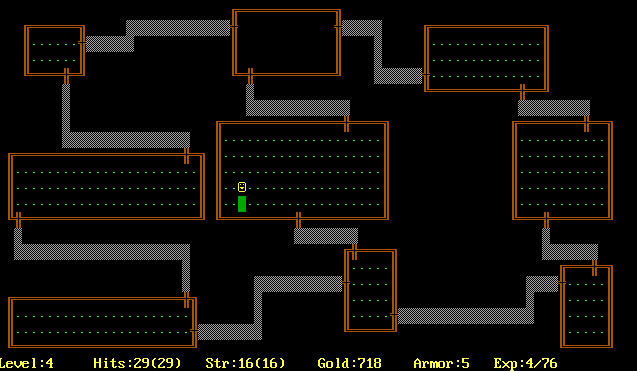
\includegraphics[scale=0.79]{Rogue.png}
\\
For an easier challenge, you may want to start with just a text based adventure.  From there you will want to 
start to design the map, and how to move your character across the screen (use positions).  You will also need to
know the ASCII characters, which are easy to look up.  Focus on the game before you focus on the graphics element
part of the challenge.

\section*{Graphics}
For graphics we will really need to use pygame.  If you do not have this installed, then I suggest doing it now.  
Basically everything will be the same as above, except that we will be using pygame will be used to gather our 
graphics and sounds.  
\\
For a simple introduction we will write the hello world program, but with graphics.

\subsection*{Graphical Hello World}
For a simple introduction we will write a graphical Hello World program.  This is going to be simple and ugly, but
it is just an introduction.  The file is located in this directory of Github.  The code is quite simple but you 
will notice that it is much more in depth than the original one line hello world we wrote before.  When we are done
we will have a window that looks like this
\\
\begin{center}
   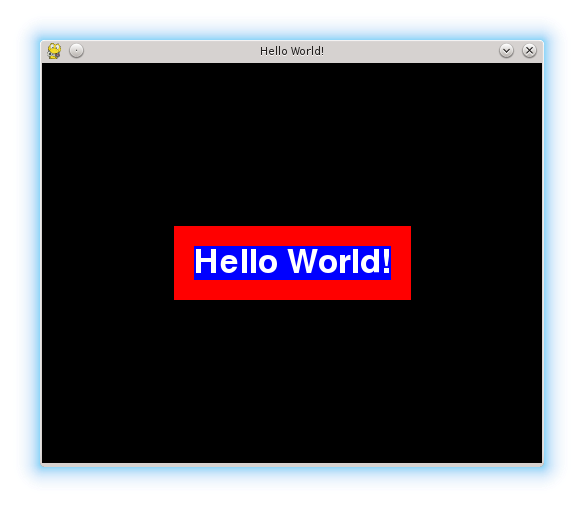
\includegraphics[scale=0.5]{HelloWorld.png}
\end{center}
\\
Though it is not nice looking, we can see that we do get a window with our desired graphics on it.  Pygame also 
allows us to draw shapes ourselves.  This can get quite tedious though and a much better option will be to 
just use pictures that were created outside.  Use GIMP, Photoshop, or whatever you like.  We will discuss this in
the next section, along with sounds.  Everything in the code should be easily readable to the student.

\subsection*{More Challenging Games}
In this section we will discuss more about graphics and sounds.


% Delete following line
Check back later for when I have completed the game.  This may take a while.  In the mean time read online if you
are more interested.
% Note about timidity++ install

\end{document}
